%\titlespacing*{\chapter}{0pt}{\baselineskip}{*3}
\chapter{Analysis}
\label{chap4}

We simultaneously model the resolved 850$\mu m$ visibilities from ALMA with the unresolved Spectral Energy Distribution (SED) in order to constrain basic geometric properties of the disk and determine the characteristics of the constituent dust grains. In Section \ref{SinglePowerSED_Model} we attempted to recreate the data with a standard power-law model of the surface density distribution of a geometrically and optically thin dust disk, and while this provided a good fit to the SED, it failed to recreate the visibilities. From the significant positive residuals apparent to the SW side of the disk and negative residuals visible near the center, it was clear that a more complex model describing the surface density was necessary. In Section \ref{MoreComplexModels}, we modeled the surface density both with a double power-law, increasing in density to a variable radius before dropping off, and with an unresolved surface density enhancement at a variable radius. Both models were able to recreate the SED, but the SED dominated the fit, skewing the fits to the visibilities. In order to create the significant mass of hot dust necessary to recreate the mid-IR excess, the best-fit results had inner radii within 1AU of the star, resulting in models that were too bright at the center. The unresolved surface density enhancement (USDE???) model was able to account for the ring-like structure, but the double power-law model was not, presumably altered by the fit to the SED. 

To eliminate the contribution of the SED, $\chi^{2}$ values were computed only using the visibilities for both the double-power law and the surface density enhancement. As presented in Section \ref{VisOnly}, we found that both models were able to recreate the density enhancement without becoming too bright at the center. However, as expected, these models didn't contribute enough flux at mid-IR wavelengths. Building upon the results of \cite{Wahh07}, we described an inner disk with a grain size of 0.1$\mu m$ and let the characteristic grain size of the outer belt vary. Because small grains radiate at higher temperatures at a given distance from the star than their larger brethren, they were able to boost the mid-IR flux without contributing significantly to the flux at millimeter wavelengths. Both the double power-law and unresolved surface density enhancement models with different characteristic grain sizes, presented in Section \ref{ThreePart}, were able to fully recreate our data. 

Best fit parameters were determined using an affine-invariant Markov Chain Monte Carlo (MCMC) fitting algorithm (\ref{Fore13}, Goodman \& Weare 2010 <<no bibtex for this??, described in Section \ref{MCMC}), a process that provides a robust, statistical characterization of the model parameters. 

A closer look at the mid-IR spectrum of 49 Ceti gathered from IRS is presented in Section \ref{MidIR}. 

%%%%%%%

\section{Single Power-law Model}
\label{SinglePowerSED_Model}

The simplest geometrically and optically-thin disk model consisted of a single power law $p$ describing the surface density profile $\Sigma(r)$, normalized to 100AU ($\Sigma_{100\text{AU}}$) and parameterized as:

\begin{equation}\label{eq:sigmaR}
\Sigma(r) = \Sigma_{100\text{AU}}\Big(\frac{r}{100\text{AU}}\Big)^{-p}
\end{equation}

We are able to solve for $\Sigma_{100\text{AU}}$, as we know the integral of the surface density over all infinitesimal rings from the inner radius, $R_{In}$, to the outer radius, $R_{Out}$ must be equal to the total mass of emitting grains in the disk, $M_{Disk}$. 

\begin{equation}\label{eq:mdisk}
M_{Disk} = \int_{R_{In}}^{R_{Out}} \Sigma(r) 2 \pi r \,dr = \int_{R_{In}}^{R_{Out}} \Sigma_{100\text{AU}}\Big(\frac{r}{100\text{AU}}\Big)^{-p} 2 \pi r \,dr
\end{equation}

Integrating and solving for $\Sigma_{100\text{AU}}$, we find:

\begin{equation}\label{eq:sigma100}
\Sigma_{100\text{AU}} = \cfrac{M_{Disk} (2 - p)}{2\pi (100\text{AU})^{p} [(R_{Out})^{2-p}-(R_{In})^{2-p}]}
\end{equation}

Equation \ref{eq:sigma100} lets us vary $p$, $R_{In}$, $R_{Out}$, and $M_{Disk}$, which, combined with equation \ref{eq:sigmaR}, lets us calculate what the surface density should be at any radius. 

The parameters that describe the dust grains are the characteristic grain size ($a$) and the long-wavelength power law index of grain emission efficiency ($\beta$). Because grains are very inefficient emitters at $\lambda$ $>>$ $2\pi a$, assigning a single grain size for the dust would be insufficient to recreate the contribution of the dust to the SED. However, modeling the quantum emission efficiency as a function of wavelength such that $Q_{\lambda} = 1 - e^{-(\frac{\lambda}{2\pi a})^{-\beta}}$ has the desired properties that $Q_{\lambda} \approx (\sfrac{\lambda}{2\pi a})^{-\beta}$ when $\lambda$ $>>$ $2\pi a$ and $Q_{\lambda} \approx 1$ when $\lambda$ $<<$ $2\pi a$, which mimics a distribution of grain sizes. Large values of $\beta$ signify an emphasis on grain sizes $\sim$ $a$, where as smaller values of $\beta$ give more weight to large grains and their emission at longer wavelengths. By smoothly describing the quantum emission efficiency in this way, we end up with a model that is very computationally efficient and is able to recreate the SED with the minimum number of variable parameters. 

%\begin{equation}\label{eq:qFn}
%$Q_{\lambda} = 1 - e^{-(\frac{\lambda}{2\pi a})^{-\beta}}$
%\end{equation}

%The combination of these parameters allows us to approximate a grain size distribution; large values of $\beta$ signify a high ratio of small grains to large grains whereas values of $\beta$ close to zero suggest .....which essentially modifies a Rayleigh-Jeans tail to approximate a distribution of grain sizes.  

The temperature of a grain of a given size at a given distance from the star can then be derived by assuming radiative equilibrium between the the solar radiation absorbed and the energy emitted by the grain. Not taking the albedo of the grains into account, the energy balance is described by:

\begin{equation}\label{EBalance}
\frac{\pi a^{2} L_{\bigstar}}{4 \pi d^{2}} = 4 \pi a^{2} \sigma T_{g}^{4}
\end{equation}

where $a$ is the grain size, $L_{\bigstar}$ is the luminosity of the central star, $d$ is the distance to the grain from the star, $\sigma$ is the Stephan-Boltzmann constant, and $T_{g}$ is the temperature of the grain. Solving for $T_{g}$, we find:

\begin{equation}\label{tEst}
T_{g} \simeq (\frac{L_{\bigstar}}{16 \pi \sigma})^{\sfrac{1}{4}} d^{\sfrac{-1}{2}}
\end{equation}

From this we can see that the temperature of the grains falls off as approximately $d^{\sfrac{-1}{2}}$. However, grains are not perfect absorbers or emitters, and the albedo changes both as a function of wavelength and grain size. To account for this, we model the composition of the dust as compact astrosilicates as described by \cite{Drai03}, and describe the grains' opacity and albedo according to Mie theory (see \citet*{Bohr83}). This allows us to derive accurate grain temperatures and their contribution to the total flux for grains throughout our model of the disk.

\begin{table*}
\caption{Unresolved Continuum Fluxes}
%\resizebox{\textwidth}{!}{
\begin{center}
%\begin{multicols*}{2}
%\setlength\columnsep{12pt}
%\def\arraystretch{1}
%\begin{tabular}{1*{5}{c}r}
\begin{tabular}{ccc}
    \hline\hline   
    Wavelength ($\mu m$) & Flux (Jy) & Source & %\multicolumn{1}{p{2cm}}{\centering Number of \\ Antennas} 
    \hline 
    0.38 & 8.68 & \cite{Sylv96} \\ 
    0.45 & 20.99 & $''$ \\    
    0.55 & 20.52 & $''$ \\     
    1.22 & 9.55 & $''$ \\     
    1.65 & 6.38 & $''$ \\     
    2.18 & 3.98 & $''$ \\     
    3.55 & 1.72 & $''$ \\     
    4.77 & 0.96 & $''$ \\
    5.86 & 0.69$\pm$0.07& IRS Spectrum \\ 
    7.07 & 0.48$\pm$0.05&$''$ \\ 
    8.97 & 0.32$\pm$0.03& $''$ \\ 
    11.40 & 0.21$\pm$0.02& $''$ \\ 
    13.90 & 0.18$\pm$0.02& $''$ \\ 
    17.13 & 0.19$\pm$0.02& $''$ \\ 
    20.90 & 0.21$\pm$0.02& $''$ \\ 
    27.21 & 0.35$\pm$0.03& $''$ \\ 
    34.00 & 0.6$\pm$0.1& $''$ \\ 
    11.56 & 20.99 & $\cite{Wrig10} \\         
    12.0 & 0.33 $\pm$ 0.07 & IRAS Faint Source Catalog \\     
    25.0 & 0.38 $\pm$ 0.08 & $''$ \\    
    60.0 & 2.0 $\pm$ 0.4 & $''$ \\     
    100.0 & 1.91 $\pm$ 0.38 & $''$ \\   
    12.5 & 0.20 $\pm$ 0.03 & \cite{Wahh07} \\   
    17.9 & 0.19 $\pm$ 0.03 & $''$ \\  
    150.0 & 0.8 $\pm$ 0.5 & ISO \\  
    170.0 & 1.1 $\pm$ 0.5 & $''$ \\  
    63.19 & 2.01 $\pm$ 0.35 & \cite{Robe13} \\
    70.00 & 2.142 $\pm$ 0.058 & $''$ \\
    72.84 & 1.95 $\pm$ 0.32 & $''$ \\
    78.74 & 1.90 $\pm$ 0.31 & $''$ \\
    90.16 & 1.88 $\pm$ 0.32 & $''$ \\
    145.54 & 1.16 $\pm$ 0.18 & $''$ \\
    157.68 & 0.98 $\pm$ 0.13 & $''$ \\
    160.00 & 1.004 $\pm$ 0.053 & $''$ \\
    250.0 & 0.372 $\pm$ 0.027 & $''$ \\
    350.0 & 0.180 $\pm$ 0.014 & $''$ \\
    500.0 & 0.086 $\pm$ 0.009 & $''$ \\
    850.0 & ???? $\pm$ ???? & This work \\
    1300.0 & 0.0021 $\pm$ 0.0008 & $''$ \\
        \hline
\end{tabular}
%    \end{multicols*}
    \end{center}
%\end{adjustbox}
\label{tab:SED}
\end{table*}


We fit our model to the SED at observed photometric points gathered from the literature (displayed in Table \ref{tab:SED}) in order to calculate a $\chi^{2}_{SED}$. The SED is modeled by two components: (1) a Kurucz-Lejeune model photosphere with surface gravity log(g)=4.5, effective temperature $T_{Eff}$=10000K, and solar metalliciity Z=0.01 (Chen et al. 2006), (2) an extended, spatially-resolved debris disk. Points at a wavelength less than 5$\mu m$ were not fit to, as the disk contributes a negligible flux relative to the star in this regime. A total of 19 points were fit to in the SED until additional photometry from \cite{Robe13} were discovered, at which point 30 points were fit to (see Section \ref{ThreePart}). The IRS spectrum originally consisted of 360 points between 5 and 35$\mu m$, but was averaged down to 9 for the sake of computational efficiency. The errors reported in the table for these points are the absolute calibration uncertainty (assumed to be 10$\%$ of the flux measurement) and the statistical uncertainty added in quadrature.

\begin{figure}[t!]
\centering
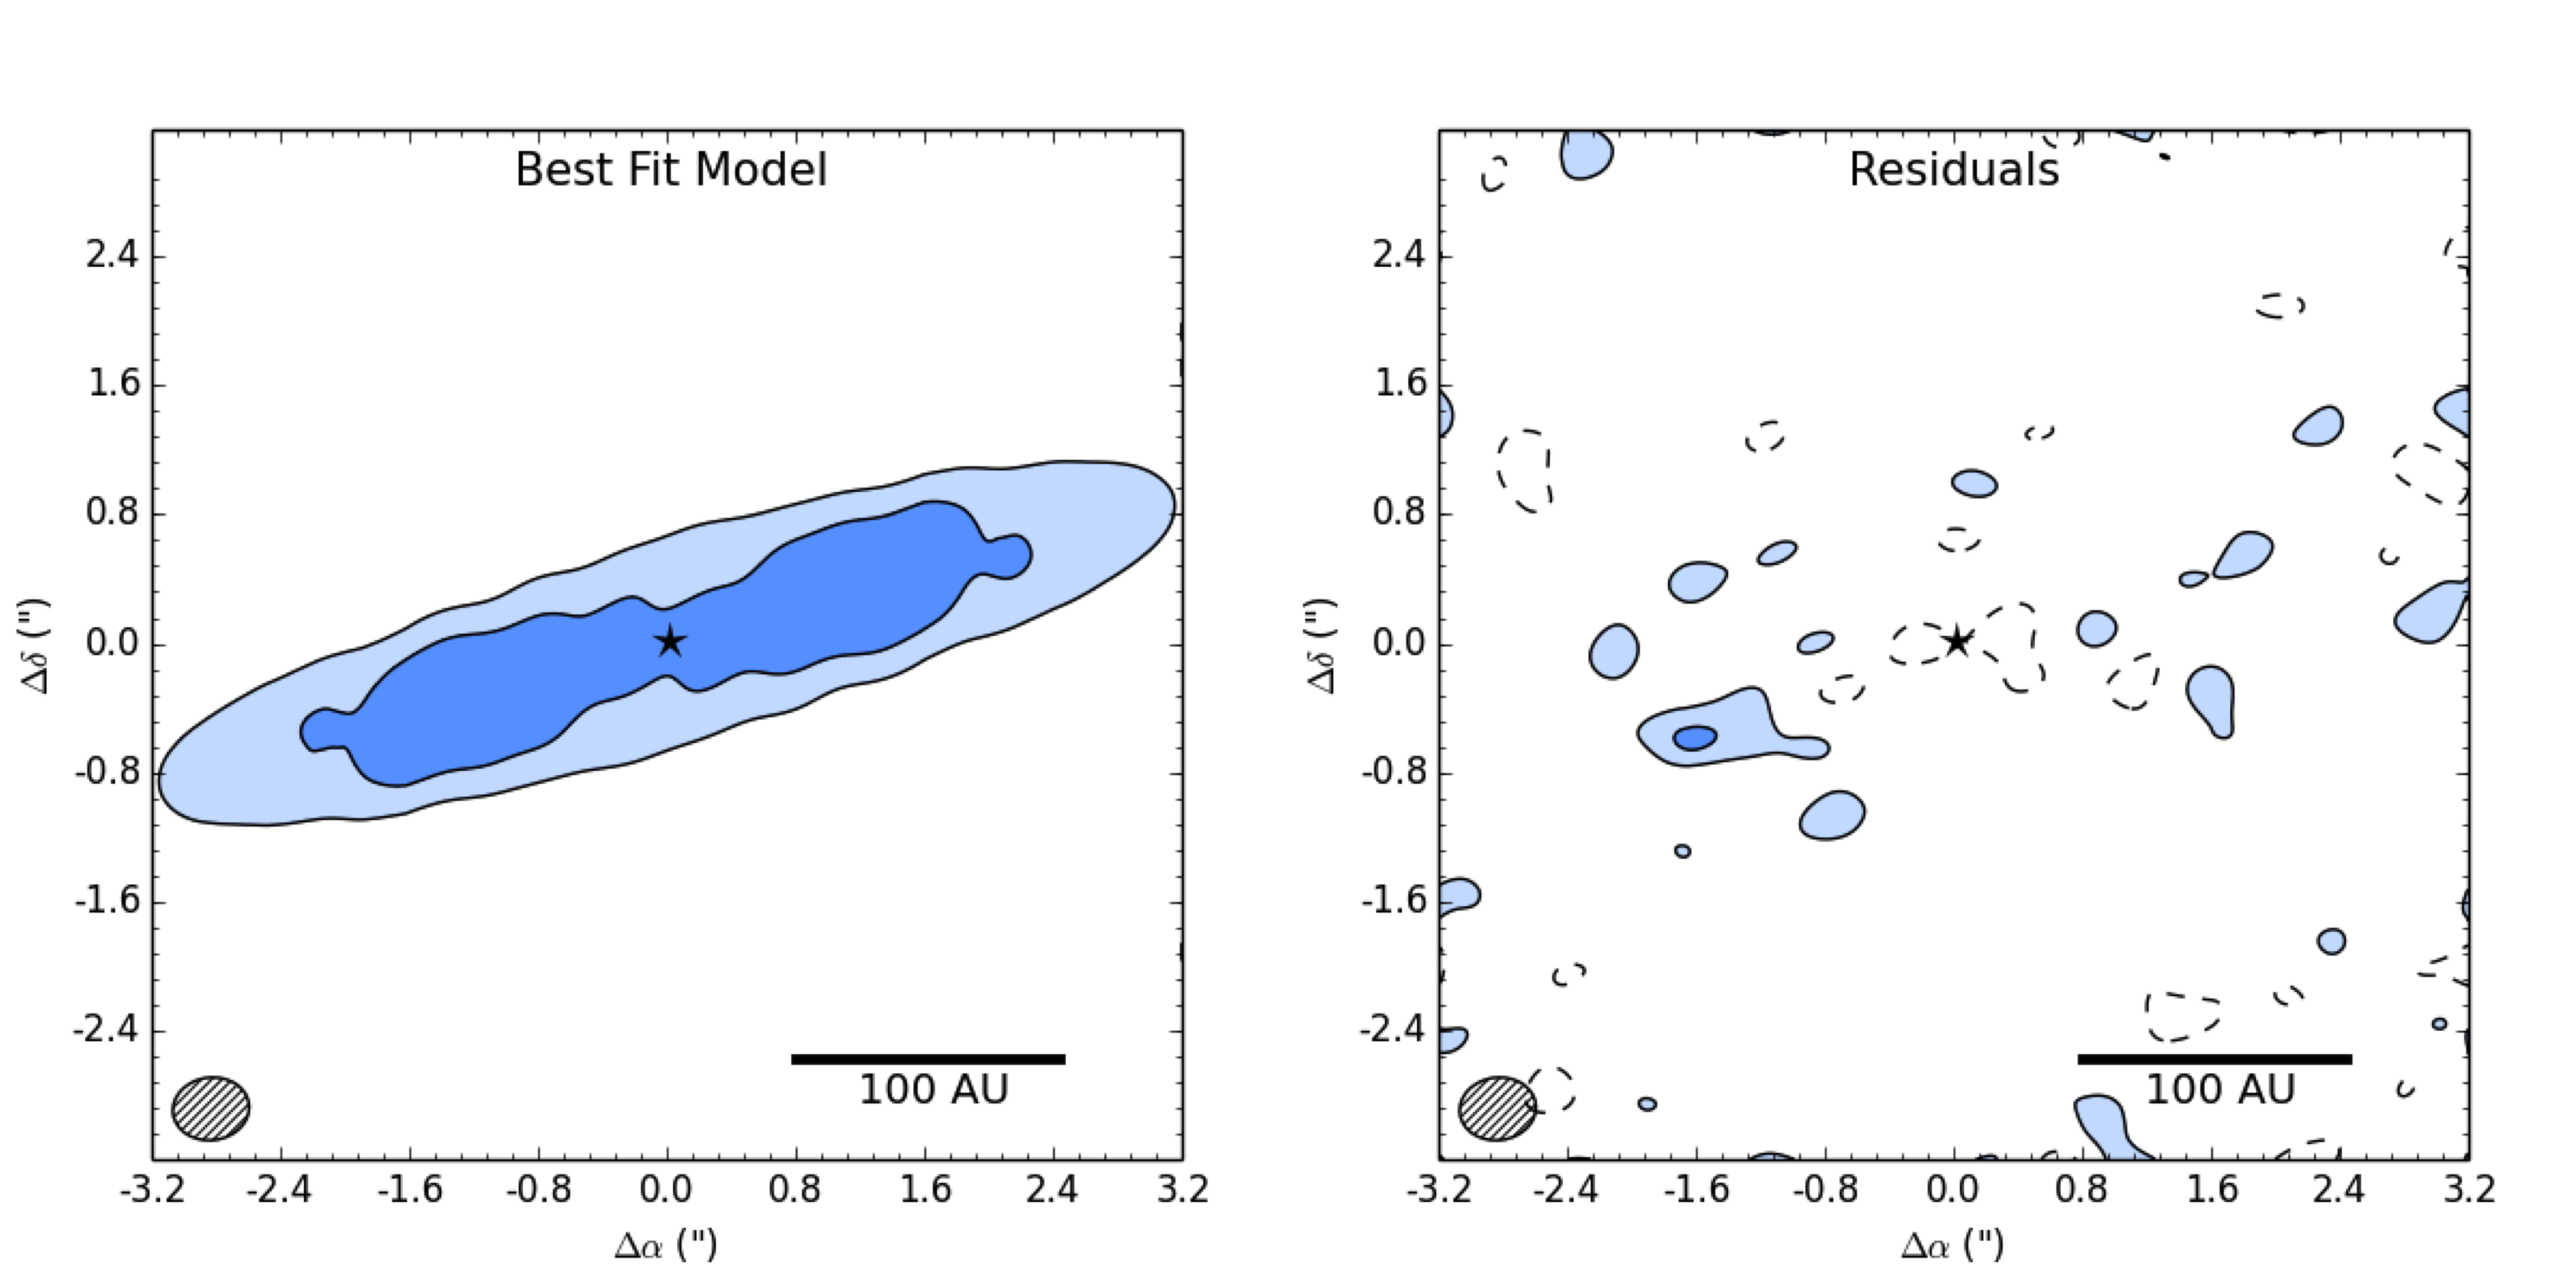
\includegraphics[width = 1\textwidth]{49CET_Simple_ModelResidual.png}
\caption{The model image (left) and residuals (right) for the single power-law model. The residuals are the ALMA visibilities minus model visibilities, subtracted in the visibility domain, then imaged. Contours are [-2, 2, 4] $\times$ 58$\mu$Jy (the RMS noise of the data image). The model fails to account for the region of higher density on the southeast side of the disk and leaves residuals in a ring-like pattern around the disk. It is also slightly too bright at the center.}
\label{fig:49CET_Simple_ModelResidual}
\end{figure}

In addition to describing and fitting the flux contribution of the grains to the SED, we simultaneously create a high-resolution model image of the disk at 850$\mu m$, the wavelength of the spatially-resolved ALMA observations. This model image is sampled at the same baseline separations and orientations as the ALMA observations with the MIRIAD command \texttt{uvmodel}, allowing us to compare our model disk to the data in the visibility domain. Although there are significantly more visibilities (141300) than SED points that we fit to (30), the visibilities have much lower signal-to-noise, meaning the weight that each $\chi^{2}$ has on the final fit is roughly equal. 

The best-fit model and residual image for the single power-law model are presented in Figure \ref{fig:49CET_Simple_ModelResidual}, and the best-fit SED is plotted in Figure \ref{fig:49CET_Simple_SED}. The model leaves 2$\sigma$ residuals in a ring, suggesting the need for a description of the surface density that peaks at a variable radius. It is also too bright near the center of the disk. The median and best-fit values for the single power-law  model are presented in Table \ref{tab:SimpleModel_Table}.

\begin{figure}[!]
\centering
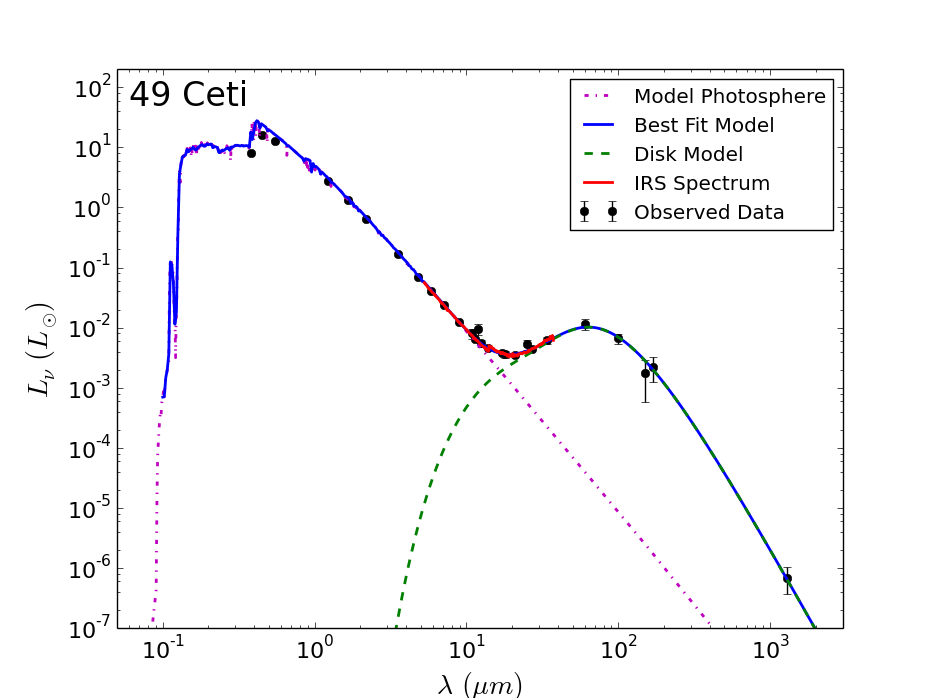
\includegraphics[width = 1\textwidth]{49CET_Simple_SED.png}
\caption{The best fit SED of 49 Ceti for the single power-law model. The best fit model is the sum of the disk model and the model photosphere. Photometric points, excluding those from \cite{Robe13}, are taken from the literature. The full IRS spectrum is presented for display purposes.}
\label{fig:49CET_Simple_SED}
\end{figure}

\begin{table}[t!]
\begin{center}
    \def\arraystretch{1.10}%
    \begin{tabular}{l*{2}{c}r}
    \hline
     Parameter & Median Value $\pm$ 1$\sigma$ & Best Fit Value \\ \hline
     $R_{In}$  [AU] & 0.82$\pm$0.10 & 0.81\\ 
     $\Delta$R [AU] & 213$\pm$6} & 212 \\ 
     log(a [$\mu$m])  & 0.63$\pm$0.10 & 0.68\\ 
     log($M_{D}$ [$M_{Earth}$])  & -0.71$\pm$0.15 & -0.63\\ 
     $\beta$ & 1.58$\pm$0.12 & 1.64\\ 
     p & -0.26$\pm$0.05 & -0.27\\ 
     i [degrees] & 79.1$\pm$0.6 & 79.4 \\ 
     PA [degrees] & -73.3$\pm$0.6 & -73.5\\
    \hline
    \end{tabular}
\caption{The median values $\pm$ 1$\sigma$ and best-fit values for the single-power law model.}
\label{tab:SimpleModel_Table}
\end{center}
\end{table}



%%%%%%%

\section{More Complex Models of the Surface Density}
\label{MoreComplexModels}

The ring-like positive residuals left by the single power-law model suggest the need for a more complex model of the surface density. We propose a double power-law model in which the surface density increases from $R_{In}$ to a transition radius $R_{T}$ before dropping off until $R_{Out}$ in section \ref{DoublePowerSED_Model} and a single power-law with a narrow, unresolved surface density enhancement in section \ref{UnresolvedDensitySED_Model}.

\subsection{The Double Power Law}
\label{DoublePowerSED_Model}

We parameterize $\Sigma(r)$ for the double power-law normalized to the surface density at the transition radius, $\Sigma_{T}$. 

\begin{equation}\label{eq:sigmaDP}
\Sigma(r) = \begin{cases}
   \Sigma_{T}\Big(\frac{r}{R_{T}}\Big)^{-p_{1}} & \text{for $R_{In}$ $\le$ r $\le R_{T}$} \\
   \Sigma_{T}\Big(\frac{r}{R_{T}}\Big)^{-p_{2}} & \text{for $R_{T}$ $\textless$ r $\le$ $R_{Out}$}
\end{cases}
\end{equation}

As earlier, we solve for $M_{Disk}$:

\begin{equation}\label{eq:mdiskDP}
\begin{flalign*}
    M_{Disk} &= \int_{R_{In}}^{R_{T}} \Sigma(r) 2 \pi r \,dr & \\
    &= \int_{R_{In}}^{R_{T}} \Sigma_{\text{T}}\Big(\frac{r}{R_{T}}\Big)^{-p_{1}} 2 \pi r \,dr & + \int_{R_{T}}^{R_{Out}} \Sigma_{\text{T}}\Big(\frac{r}{R_{T}}\Big)^{-p_{2}} 2 \pi r \,dr &&
\end{flalign*}
\end{equation}

We integrate and solve for $\Sigma_{T}$, defining $j_{1} = 2 - p_{1}$, $j_{2} = 2 - p_{2}$, $m_{1} = R_{T}^{j_{1}} - R_{In}^{j_{1}$, and $m_{2} = R_{Out}^{j_{2}} - R_{T}^{j_{2}$ for readability:

\begin{equation}\label{eq:sigmaT}
\Sigma_{T} = \cfrac{M_{Disk} (j_{1} j_{2})}{2\pi [(m_{1} j_{2})(R_{T})^{p_{1}} + (m_{2} j_{1})(R_{T})^{p_{2}}]}
\end{equation}

This parameterization of $\Sigma_{T}$ allows us to vary $R_{In}$, $R_{T}$, $R_{Out}$, $M_{Disk}$, $p_{1}$, and $p_2$ in our search for a best-fit model. We use $a$ and $\beta$ to describe the population of grains and $i$ and $PA$ to describe the geometry on the sky as in the single power-law model. 

\begin{figure}
\centering
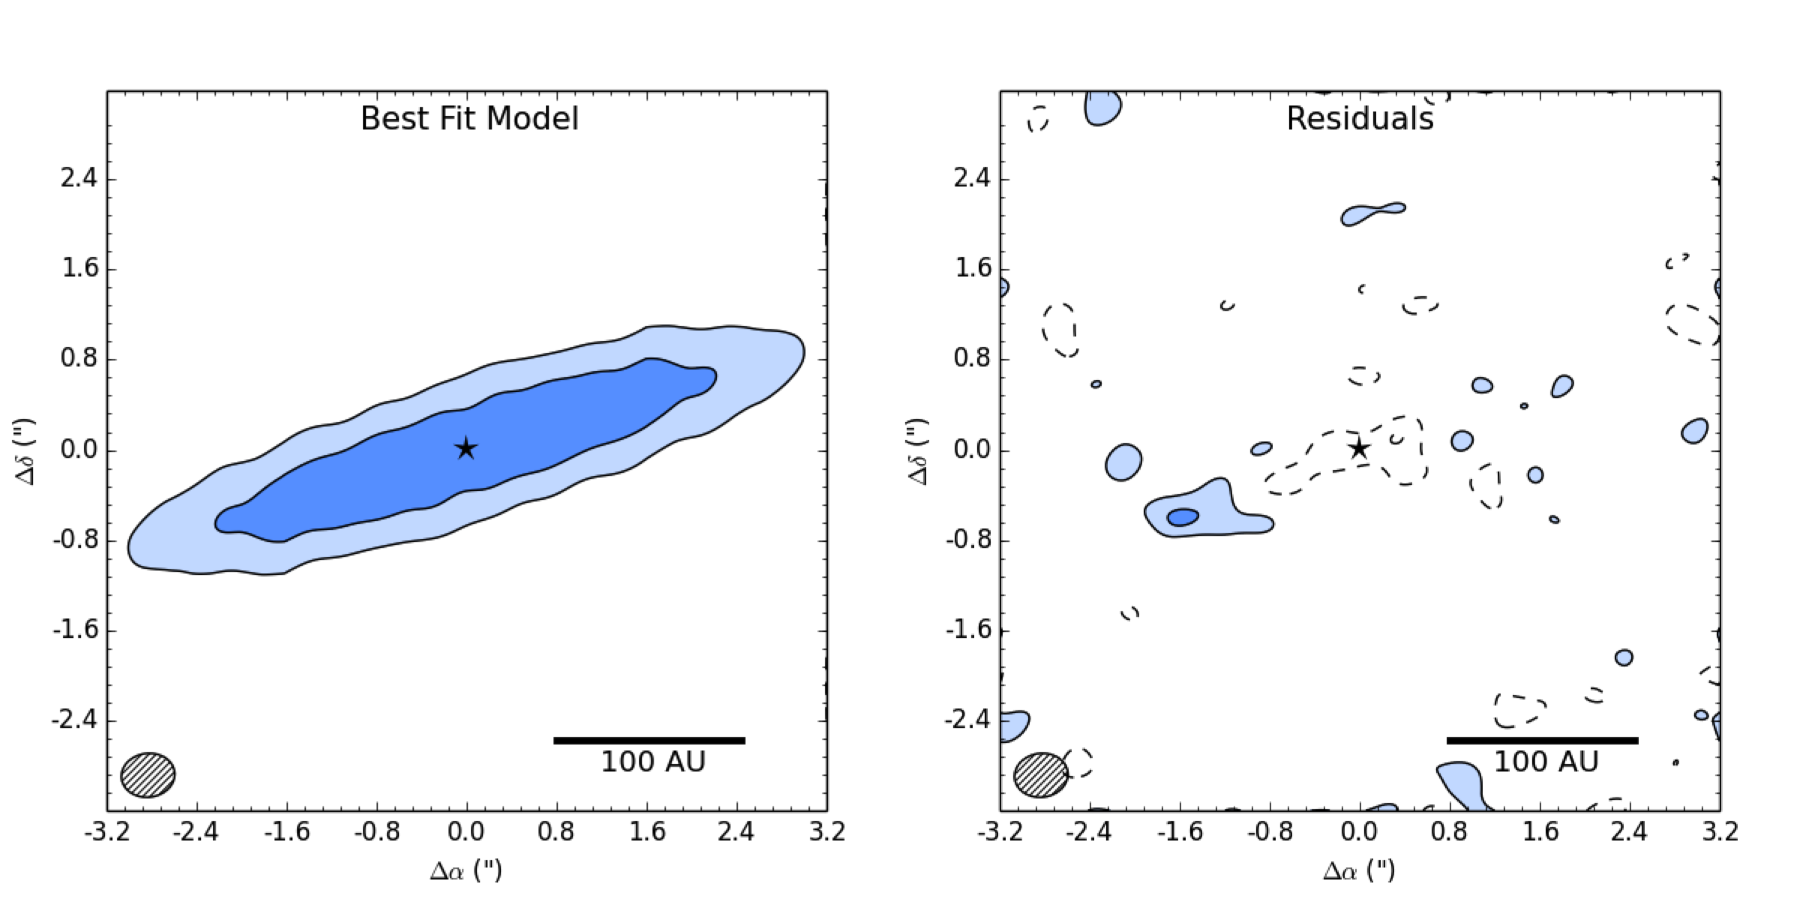
\includegraphics[width = 1\textwidth]{49CET_DoublePowerSED_ModelResidual.png}
\caption{The model image (left) and residuals (right) for the double power-law model, simultaneously fitting the SED and the visibilities. Contours are [-4, -2, 2, 4] $\times$ 58$\mu$Jy. The model fails to account for the region of high density on the southeast side of the disk and is much too bright at the center, but does get rid of the ring-like 2$\sigma$ residuals left by the single power-law model.}
\label{fig:49CET_DoublePowerSED_ModelResidual}
\end{figure}

\begin{table}
\begin{center}
    \def\arraystretch{1.37}%
    \begin{tabular}{l*{2}{c}r}
    \hline
    Parameter & Median Value $\pm$ 1$\sigma$ & Best Fit Value \\ \hline
     $R_{In}$  [AU] & 1.15$^{+0.10}_{-0.08}$ & 1.12\\  
     $\Delta R_{In}$ [AU] & 136$^{+8}_{-6}$ & 137\\ 
     $\Delta R_{Out}$ [AU] & 191$^{+4}_{-3}$ & 191\\ 
     log($M_{Disk}$ [$M_{Earth}$]) & -1.40$^{+0.01}_{-0.01}$ & -1.40 \\
     log(a [$\mu$m]) & 0.36$^{+0.02}_{-0.02}$ & 0.36\\ 
     $\beta$ & 1.24$^{+0.02}_{-0.02}$ & 1.24\\ 
     $p1$ & -0.23$^{+0.04}_{-0.04}$ & -0.25\\ 
     $p2$ & 1.4$^{+0.2}_{-0.2}$ & 1.4\\ 
     $i$ [$^\circ$] & 78.8$^{+0.2}_{-0.2}$ & 78.7 \\ 
     $PA$ [$^\circ$] & -72.0$^{+0.4}_{-0.5}$ & -72.0\\
    \hline
    \end{tabular}
\end{center}
\caption{The median and best fit values for the double power law model, simultaneously fitting the SED and the visibilities. NOTE: I WILL PROBABLY REPORT $R_{T}$ RATHER THAN $\Delta R_{In}$} 
%of 49 Ceti's dust disk, THIS IS DOUBLE POWER with NO asteroidbelt at all, 6x1300}
\label{tab:doublePowerSEDTable}
\end{table}

The best-fit model values as well as the most likely model values derived from the MCMC chain are displayed in Table \ref{tab:doublePowerSEDTable}, and the best-fit model and corresponding residuals are displayed in Figure \ref{fig:49CET_DoublePowerSED_ModelResidual}. This model was a good fit to the SED (not displayed), but it failed to account for the region of higher density on the southeast side apparent in the resolved ALMA data. In addition, it is brighter at the center of the disk than even the simple power-law model, as can be seen from the larger area of -2$\sigma$ residuals near the star. However, this model succeeds at getting rid of much of the ring-like 2$\sigma$ residuals left by the single power-law model.

The double power-law model's attempt to simultaneously recreate the SED and visibilities forces $R_{In}$ to smaller radii and flattens $p_{1}$ in order to have enough hot grains to recreate the mid-IR excess. While this allows the model to fit to the SED, its effect on the fit to the visibilities suggests another modeling strategy is necessary.


\subsection{The Unresolved Density Enhancement}
\label{UnresolvedDensitySED_Model}

Describing the region of higher density with a narrow, unresolved belt, which doesn't have the requirement of slowly ramping up in surface density before dropping off like in the double power-law model, does better at simultaneously fitting the SED and the visibilities. This belt, which we model to be 3AU wide at a distance $R_{Belt}$ and of mass $M_{Belt}$, exists on top of a broad, single power-law description of the surface density from $R_{In}$ to $R_{Out}$ as described in Section \ref{SinglePowerSED_Model}. 

The best-fit model and residuals are displayed in Figure \ref{fig:49CET_BonusBeltSED_ModelResidual}, and the table of values derived from the MCMC chain is presented in Table \ref{tab:49CET_BonusBeltSED_Table}. The best-fit SED is shown in Figure \ref{fig:49CET_BonusBeltSED_SED}, with separate contributions to the total flux of the model displayed for the broad disk described by the single power-law and by the additional belt. While the IR excess is dominated by the disk model, the belt contributes a non-negligible flux to the SED, both at the IR excess peak of $\sim$ 70$\mu m$ and at the wavelength of the ALMA image (850$\mu m$). 
\begin{figure}%[t!]
\label{fig:49CET_BonusBeltSED_SED}
\centering
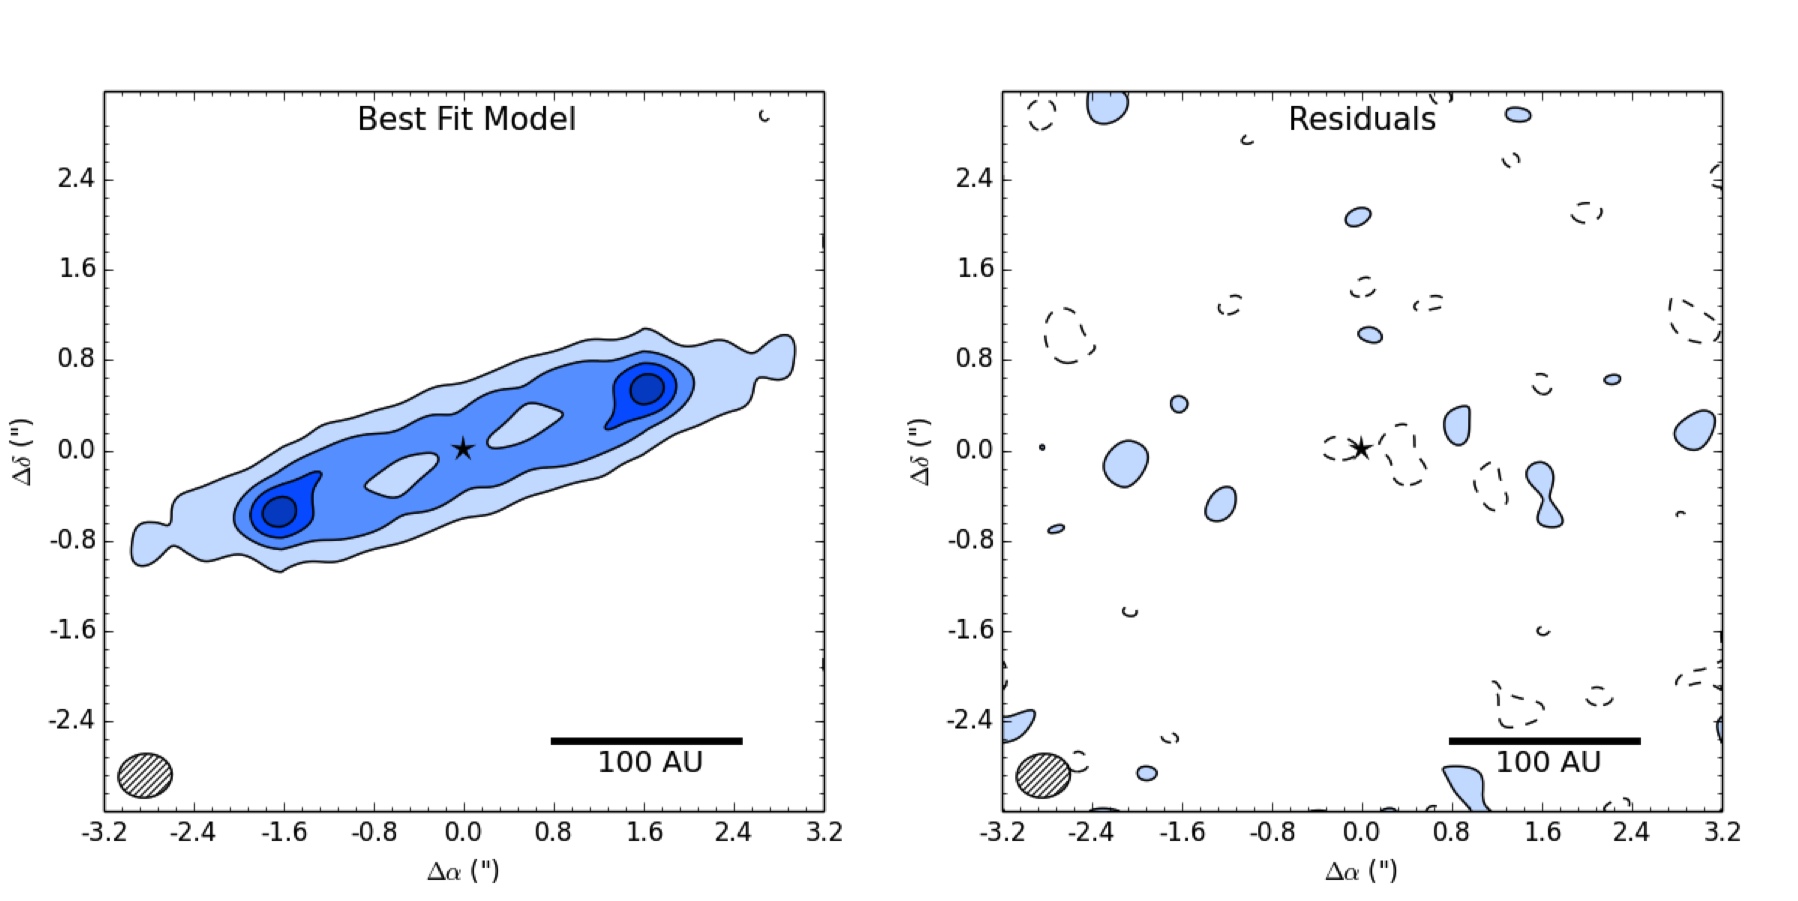
\includegraphics[width = 1\textwidth]{49CET_BonusBeltSED_ModelResidual.png}
\caption{The model image (left) and residuals (right) for the unresolved surface density enhancement model, simultaneously fitting the SED and the visibilities. Contours are [-2, 2, 4, 6, 8] $\times$ 58$\mu$Jy. The model successfully takes care of the region of high density on the southeast side of the disk, but is still slightly too bright at the center.}
\label{fig:49CET_BonusBeltSED_ModelResidual}
\end{figure}
\begin{figure}%[t!]
\centering
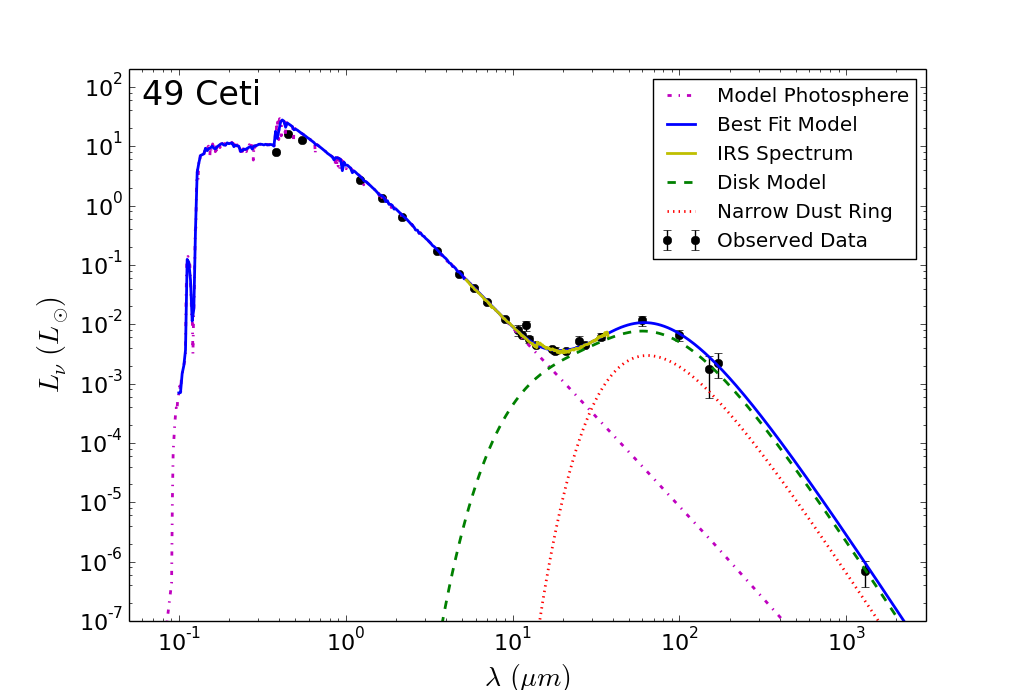
\includegraphics[width = 1\textwidth]{49CET_BonusBeltSED_SED.png}
\caption{The best fit SED of 49 Ceti for the unresolved surface density enhancement model. The best fit model is the sum of the disk model, the model photosphere, and the DENSE DUST BELT (CHANGE THIS FIND THE OTHER PLOT!).}
\label{fig:49CET_BonusBeltSED_SED}
\end{figure}
\begin{table}
\begin{center}
    \def\arraystretch{1.37}%
    \begin{tabular}{l*{2}{c}r}
    \hline
    Parameter & Median Value $\pm$ 1$\sigma$ & Best Fit Value \\ \hline
     $R_{In}$  [AU] & 1.3$^{+0.7}_{-0.5}$ & 1.3\\  
     $\Delta R$ [AU] & 290$^{+8}_{-7}$ & 291\\ 
     log($M_{Disk}$ [$M_{Earth}$]) & -1.1$^{+0.2}_{-0.2}$ & -1.1 \\
     $R_{Belt}$  [AU] & 112$^{+2}_{-2}$ & 112\\ 
     log($M_{Belt}$ [$M_{Earth}$]) & -1.8$^{+0.2}_{-0.2}$ & -1.7\\
     log(a [$\mu$m]) & 0.27$^{+0.17}_{-0.19}$ & 0.31\\ 
     $\beta$ & 1.25$^{+0.15}_{-0.12}$ & 1.27\\ 
     $p$ & -0.11$^{+0.06}_{-0.06}$ & -0.07\\ 
     $i$ [$^\circ$] & 79.5$^{+0.4}_{-0.4}$ & 79.5 \\ 
     $PA$ [$^\circ$] & -71.0$^{+0.4}_{-0.4}$ & -71.0\\
    \hline
    \end{tabular}
\end{center}
\caption{The median and best fit values for the unresolved density enhancement model.}
%for all parameters of the model of 49 Ceti's dust disk. THIS IS SIMPLE BONUS BELT, VIS & SED 120x842 WITH CORRECT UNCERTAINTIES}
\label{tab:49CET_BonusBeltSED_Table}
\end{table}
%The total best-fit mass for this model is 0.10 $M_{Earth}$, whereas the simple power-law model had a mass of 0.23$M_{Earth}$
%The best-fit value of $p$ shows that the disk is nearly flat, whereas

This model does a better job at recreating the density enhancement in the disk and still fitting to the SED, but just like with the double power-law model, it is too bright at the center. As earlier, in order to create grains hot enough to boost the mid-IR flux with only one characteristic grain size population, the inner radius of the disk is pushed inward to ~1AU. These grains are then able to recreate the mid-IR excess, but in doing so contribute too much flux at the wavelength of the ALMA image, resulting in a model that is too bright near the star.


%%%%%

\section{Visibility-only Fits}
\label{VisOnly}

To see how strongly the SED was altering the best-fit models, we ran fits with MCMC based just on the visibility $\chi^{2}$. We find that both the double power-law and unresolved surface density enhancement models are able to recreate the visibilities, and that differences between parameters between the two models are not significant. This is clear both from the minimal leftovers in each residual image and from an F-test, which confirmed that neither model is better the other in a statistically significant way.

Both models settle on approximately the same radius for the peak of the surface density. $R_{T}$ = 105AU for the double power-law model, and $R_{Belt}$ = 113AU for the unresolved surface density enhancement model. Without the simultaneous fit to the SED, $M_{Disk}$, $\beta$, and $a$ are not well constrained.

\subsection{The Double Power Law}
\label{DoublePowerVis_Model}

The best-fit model and residual images are presented in Figure \ref{fig:49CET_DoublePowerVIS_ModelResidual} and values derived from the MCMC chain are displayed in Table \ref{tab:49CET_DoublePowerVIS_Table}. Although the best-fit inner radius of this model is still close to the star ($\sim$ 6AU), it ramps up toward $R_{T}$ much more steeply. Using the double power-law model but simultaneously fitting to the SED and visibilities resulted in a best-fit value for $p_{1}$ of $-$0.25, whereas fitting just the visibilities resulted in $p_{1} = -1.76$ (remember that negative values of p are increasing, as $\Sigma \propto r^{-p}$). This means that the model from the visibility fit is much less bright at small radii than in the simultaneous fit, and this is apparent in the significantly smaller area of negative residuals around the star. In addition, this model, not under the influence of the SED, is able to recreate the region of higher density. 

\begin{figure}
\centering
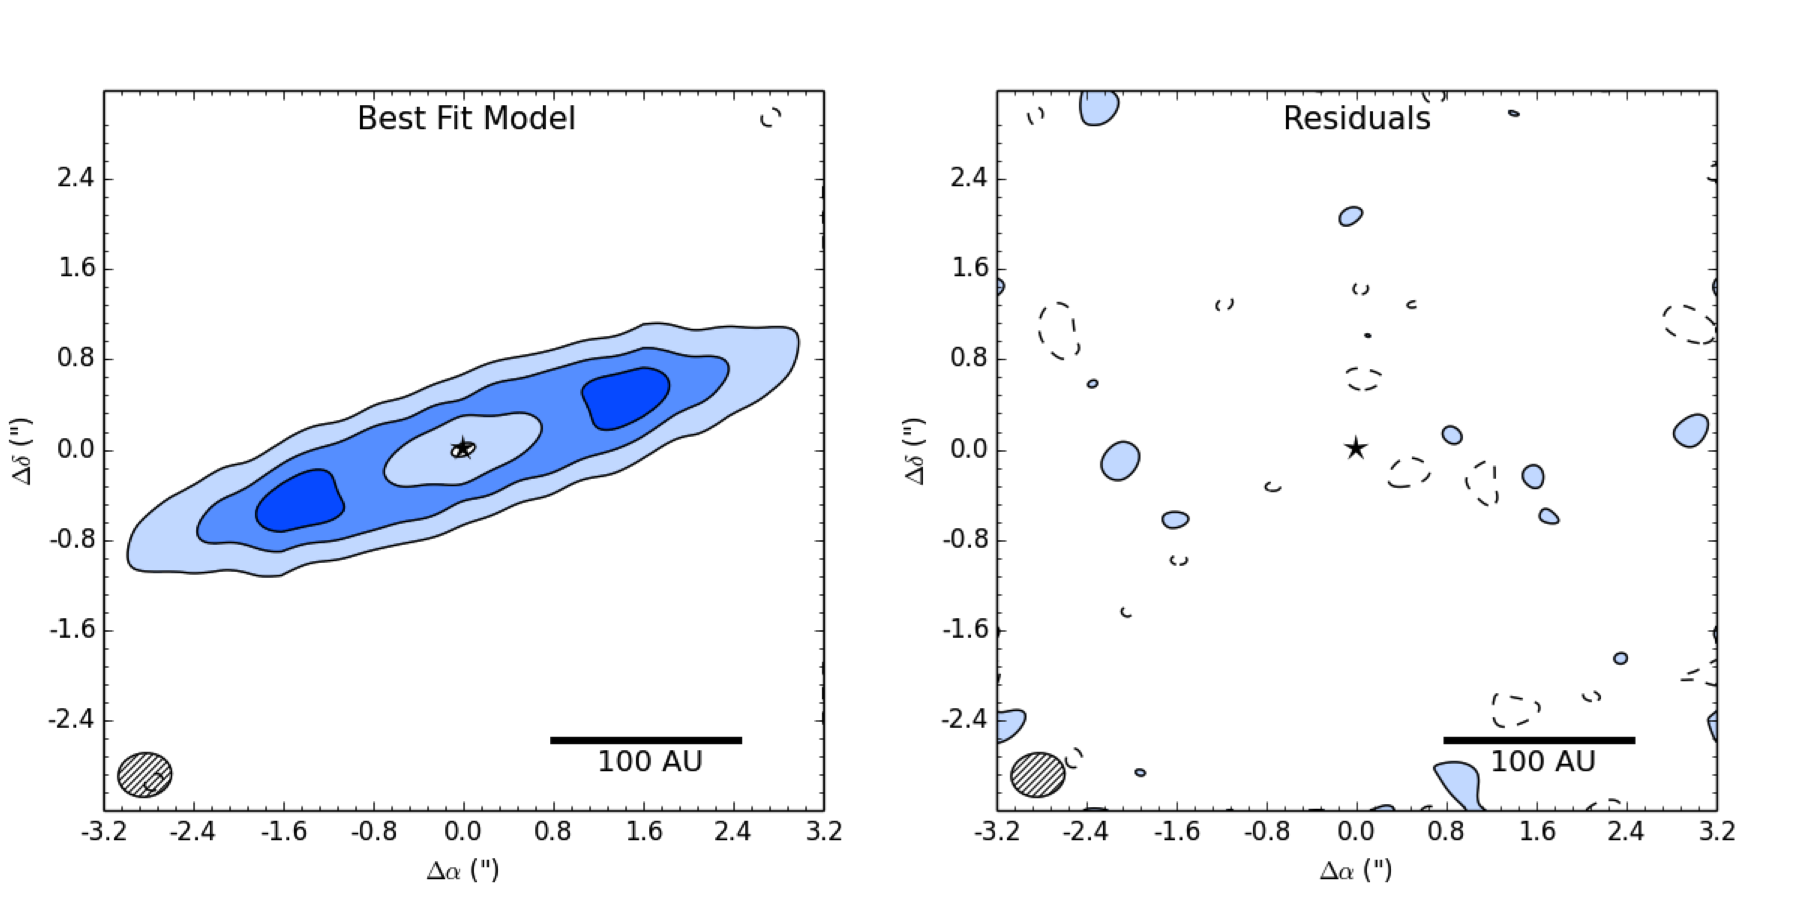
\includegraphics[width = 1\textwidth]{49CET_DoublePowerVIS_ModelResidual.png}
\caption{The model image (left) and residuals (right) for the double power-law model fitting just the visibilities. Contours are [-2, 2, 4, 6] $\times$ 58$\mu$Jy. The model leaves only a small scatter of 2$\sigma$ residuals.}
\label{fig:49CET_DoublePowerVIS_ModelResidual}
\end{figure}

\begin{table}
\begin{center}
    \def\arraystretch{1.37}%
    \begin{tabular}{l*{2}{c}r}
    \hline
    Parameter & Median Value $\pm$ 1$\sigma$ & Best Fit Value \\ \hline
     $R_{In}$  [AU] & 26$^{+20}_{-17}$ & 6\\  
     $\Delta R_{T}$ [AU] & 78$^{+16}_{-17}$ & 99\\ 
     $\Delta R_{Out}$ [AU] & 215$^{+13}_{-12}$ & 212\\ 
     log($M_{Disk}$ [$M_{Earth}$]) & -1.4$^{+0.5}_{-0.5}$ & -2.2 \\
     log(a [$\mu$m]) & 0.5$^{+0.4}_{-0.4}$ & 0.4\\ 
     $\beta$ & 1.4$^{+0.3}_{-0.3}$ & 0.8\\ 
     $p1$ & -1.7$^{+0.6}_{-0.6}$ & -1.8\\ 
     $p2$ & 1.52$^{+0.19}_{-0.16}$ & 1.55\\ 
     $i$ [$^\circ$] & 79.2$^{+0.4}_{-0.4}$ & 79.1 \\ 
     $PA$ [$^\circ$] & -71.7$^{+0.5}_{-0.5}$ & -71.5\\
    \hline
    \end{tabular}
\end{center}
\caption{The median and best fit values for the double power law model fitting only the visibilities.}
% for all parameters of the model of 49 Ceti's dust disk, THIS IS DOUBLE POWER VIS ONLY 100x600}
\label{tab:49CET_DoublePowerVIS_Table}
\end{table}


\subsection{The Unresolved Density Enhancement}
\label{UnresolvedDensityVIS_Model}

Unlike the double power-law model, fitting to just the visibilities with the best-fit unresolved density enhancement model resolves the inner radius of the disk to be 56AU (See Table \ref{tab:49CET_BonusBeltVIS_Table}), whereas the double power-law model settled on a best-fit of 6AU. This larger value for $R_{In}$ is visible in the best-fit model image (Figure \ref{fig:49CET_BonusBeltVIS_ModelResidual}), as there is no emission next to the star. However, this difference has no effect on the residual image map, which shows basically the same scatter of -2$\sigma$ residuals as in the double power-law best-fit residual image. 

\begin{figure}
\centering
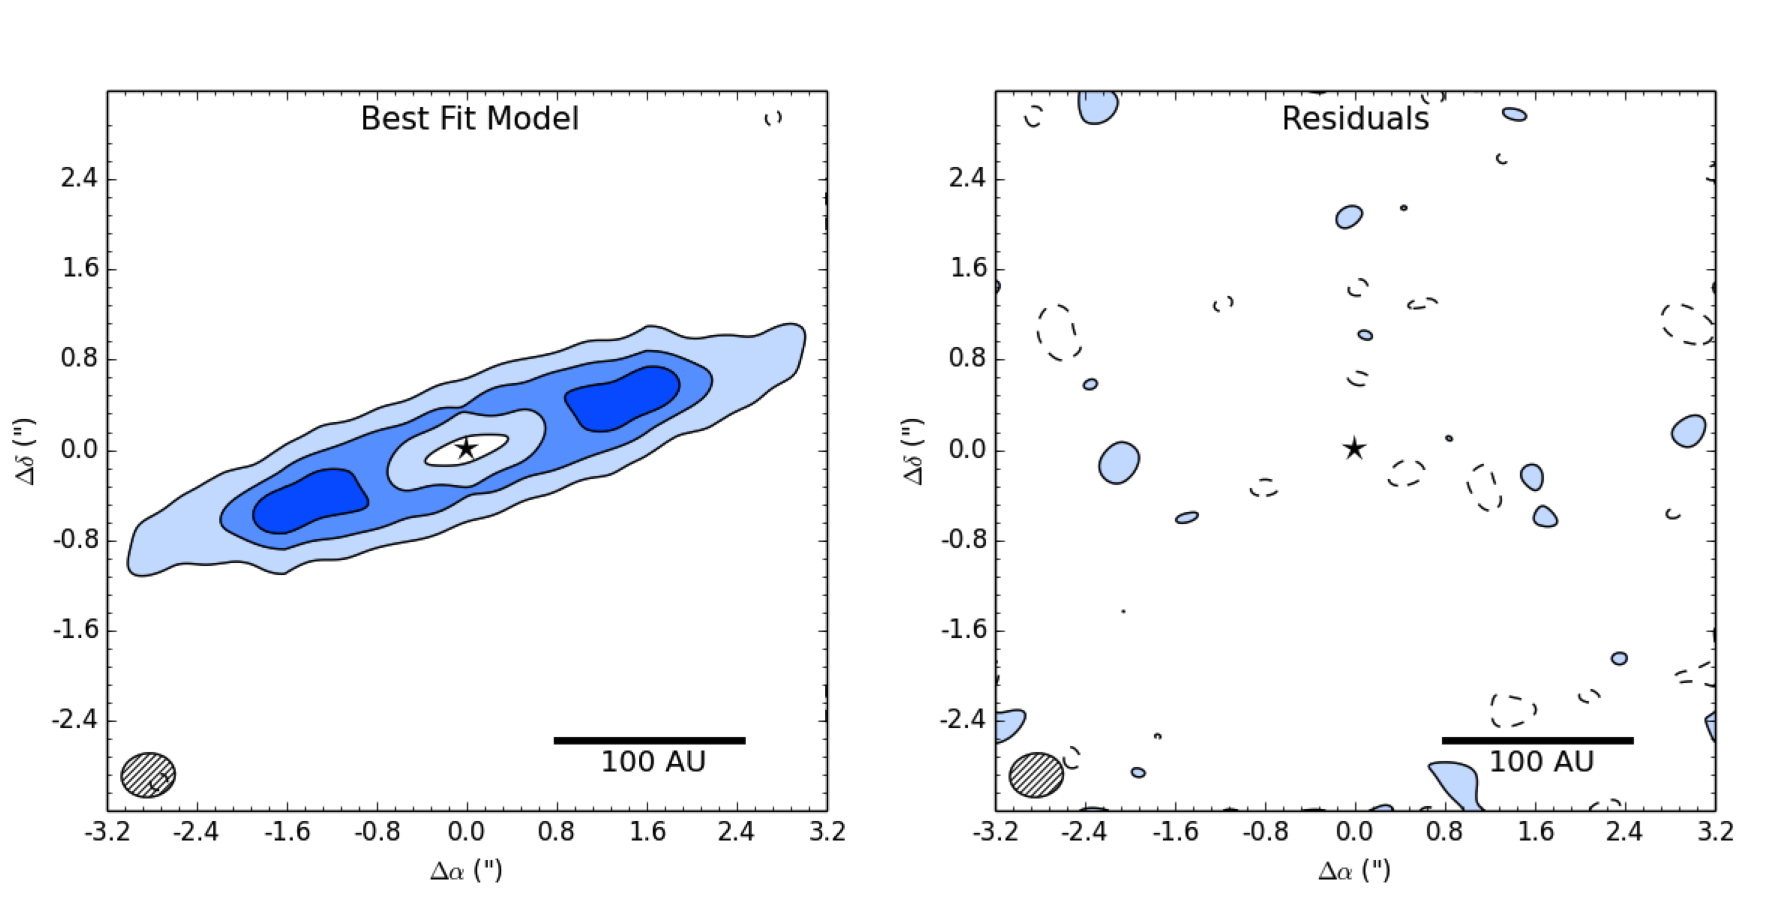
\includegraphics[width = 1\textwidth]{49CET_BonusBeltVIS_ModelResidual.png}
\caption{The model image (left) and residuals (right) for the unresolved surface density enhancement model fitting just the visibilities. Contours are [-2, 2, 4, 6] $\times$ 58$\mu$Jy. The model leaves only a small scatter of 2$\sigma$ residuals.}
\label{fig:49CET_BonusBeltVIS_ModelResidual}
\end{figure}

\begin{table}
\begin{center}
    \def\arraystretch{1.37}%
    \begin{tabular}{l*{2}{c}r}
    \hline
    Parameter & Median Value $\pm$ 1$\sigma$ & Best Fit Value \\ \hline
     $R_{In}$  [AU] & 58$^{+6}_{-6}$ & 56\\  
     $\Delta R$ [AU] & 248$^{+8}_{-8}$ & 252\\ 
     log($M_{Disk}$ [$M_{Earth}$]) & -0.8$^{+0.5}_{-0.9}$ & -0.7 \\
     $R_{Belt}$  [AU] & 114$^{+3}_{-3}$ & 113\\ 
     log($M_{Belt}$ [$M_{Earth}$]) & -1.9$^{+0.6}_{-0.8}$ & -1.6\\
     log(a [$\mu$m]) & 0.3$^{+0.9}_{-0.7}$ & -0.1\\ 
     $\beta$ & 1.4$^{+0.4}_{-0.4}$ & 1.4\\ 
     $p$ & 0.6$^{+0.4}_{-0.4}$ & 0.6\\ 
     $i$ [$^\circ$] & 79.4$^{+0.4}_{-0.4}$ & 79.4 \\ 
     $PA$ [$^\circ$] & -71.2$^{+0.4}_{-0.6}$ & -71.1\\
    \hline
    \end{tabular}
\end{center}
\caption{The median and best fit values for the unresolved density enhancement model fitting only the visibilities.}
\label{tab:49CET_BonusBeltVIS_Table}
%for all parameters of the model of 49 Ceti's dust disk. THIS IS SIMPLE BONUS BELT, JUST VIS100x840}
\end{table}


%%%%%%

\section{SED and Visibility Fits with a Three Part Disk Model}
\label{ThreePart}

\subsection{DPMODEL}
\label{dunno}

\begin{table}
\begin{center}
    \def\arraystretch{1.37}%
    \begin{tabular}{l*{2}{c}r}
    \hline
    Parameter & Median Value $\pm$ 1$\sigma$ & Best Fit Value \\ \hline
     $R_{In}$  [AU] & 4.0$^{+1.3}_{-1.0}$ & 3.4\\  
     $\Delta R_{Inner Disk}$ [AU] & 45$^{+9}_{-11}$ & 37\\ 
     $\Delta R_{T}$ [AU] & 51$^{+12}_{-9}$ & 59\\ 
     $\Delta R_{Out}$  [AU] & 222$^{+11}_{-13}$ & 216\\ 
     log($M_{Inner Disk}$ [$M_{Earth}$]) & -4.64$^{+0.15}_{-0.19}$ & -4.81 \\
     log($M_{Outer Disk}$ [$M_{Earth}$]) & -1.76$^{+0.11}_{-0.11}$ &-1.72 \\
     log(a [$\mu$m]) & 0.08$^{+0.11}_{-0.12}$ & 0.10\\ 
     $\beta$ & 1.16$^{+0.06}_{-0.05}$ & 1.18\\ 
     $p_{1}$ & -1.9$^{+0.8}_{-1.4}$ & -2.0\\ 
     $p_{2}$ & 1.47$^{+0.15}_{-0.14}$ & 1.48\\ 
     $i$ [$^\circ$] & 79.3$^{+0.4}_{-0.4}$ & 79.2 \\ 
     $PA$ [$^\circ$] & -71.5$^{+0.4}_{-0.5}$ & -71.3\\
    \hline
    \end{tabular}
\end{center}
\caption{This is dPBAG 40x800}
\end{table}
%dPBAG 40x800 SED+VIS (correct sig fig) }


\begin{figure}
\centering
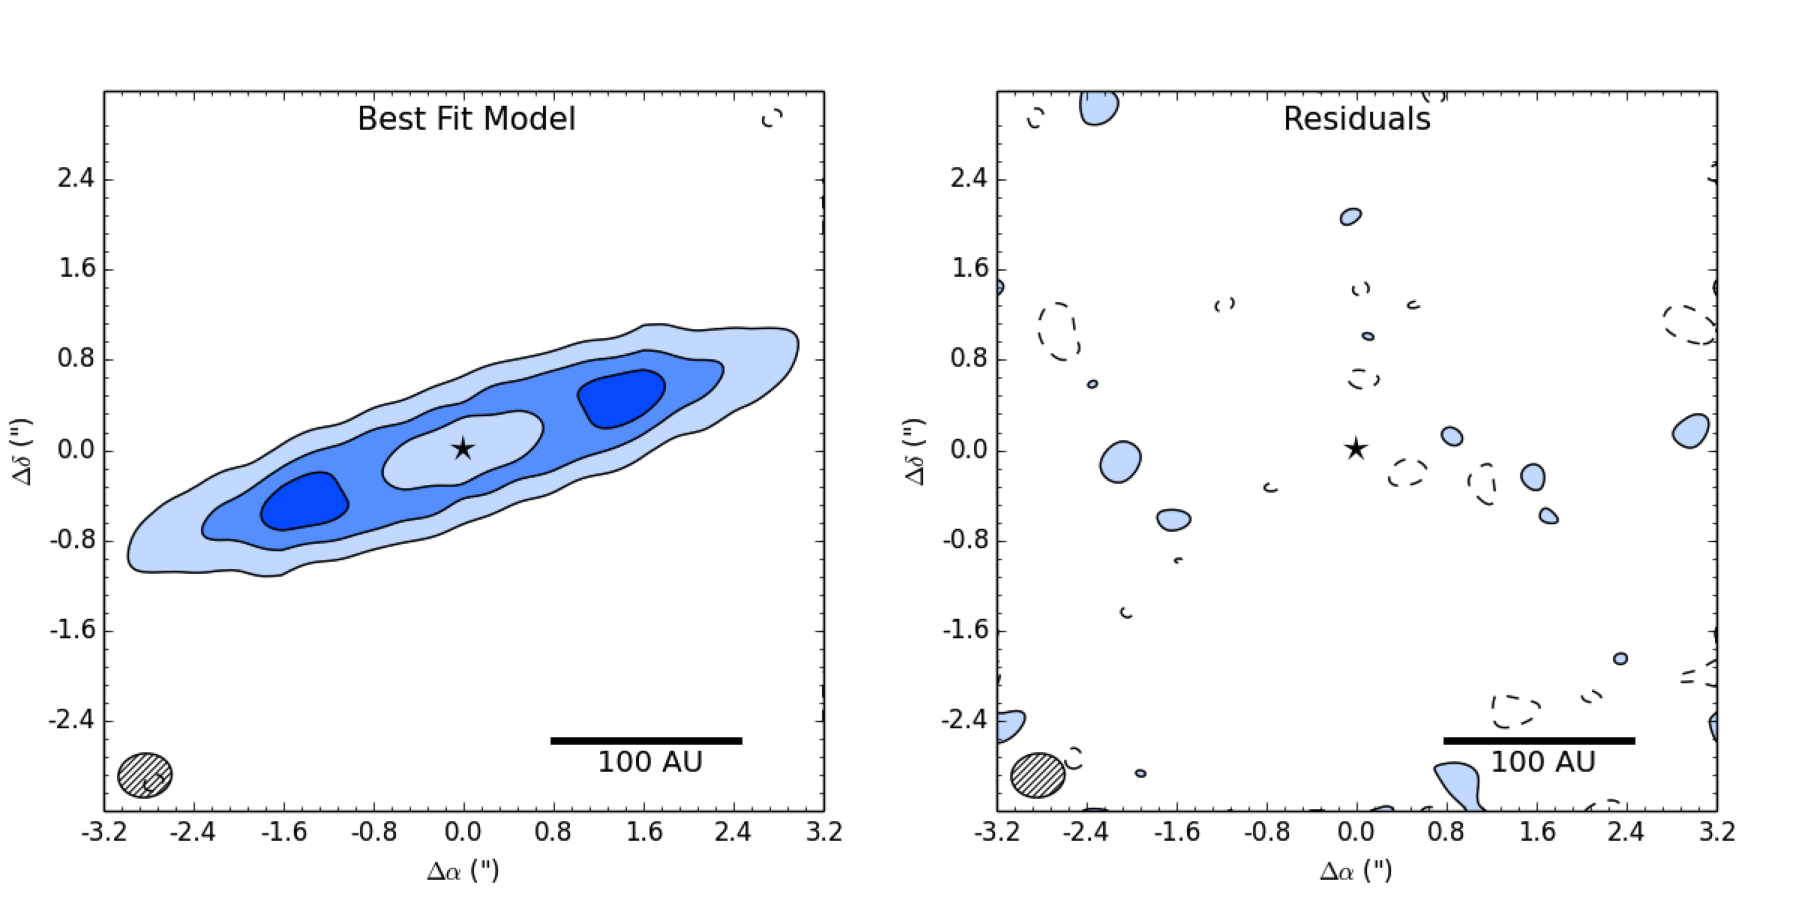
\includegraphics[width = 1\textwidth]{49CET_dPBAG_ModelResidual.png}
\caption{The model image (left) and residuals (right) for the double power law with an an additional inner disk of small grains. Contours are [-2, 2, 4, 6] $\times$ 58$\mu$Jy. The model leaves only a small scatter of 2$\sigma$ residuals. SOMETHING ABOuT NO 2sig in center}
\label{fig:49CET_dPBAG_ModelResidual}
\end{figure}

\subsection{SurfaceDensityBump}
\label{dunno}

Transition radius = transition radius
outer radius = inner radius + delta rOut

\begin{table}
\begin{center}
    \def\arraystretch{1.37}%
    \begin{tabular}{l*{2}{c}r}
    \hline
    Parameter & Median Value $\pm$ 1$\sigma$ & Best Fit Value \\ \hline
     $R_{In}$  [AU] & 4.6$^{+1.5}_{-1.2}$ & 3.5\\  
     $\Delta R_{Out}$ [AU] & 302$^{+9}_{-8}$ & 303\\ 
     $R_{Transition}$ [AU] & 62$^{+5}_{-5}$ & 60\\ 
     $R_{Ring}$  [AU] & 114$^{+3}_{-3}$ & 114\\ 
     log($M_{Inner Disk}$ [$M_{Earth}$]) & -3.3$^{+0.2}_{-0.2}$ & -3.4 \\
     log($M_{Outer Disk}$ [$M_{Earth}$]) & -1.21$^{+0.09}_{-0.10}$ &-1.21 \\
     log($M_{Ring}$ [$M_{Earth}$]) & -2.26$^{+0.15}_{-0.18}$ &-2.26 \\
     log(a [$\mu$m]) & 0.09$^{+0.10}_{-0.13}$ & 0.06\\ 
     $\beta$ & 1.17$^{+0.05}_{-0.05}$ & 1.17\\ 
     $p$ & 0.80$^{+0.19}_{-0.17}$ & 0.75\\ 
     $i$ [$^\circ$] & 79.3$^{+0.4}_{-0.4}$ & 79.3 \\ 
     $PA$ [$^\circ$] & -71.4$^{+0.4}_{-0.4}$ & -71.2\\
    \hline
    \end{tabular}
\end{center}
\caption{bBBAG 100x1200}
\end{table}

\begin{figure}
\centering
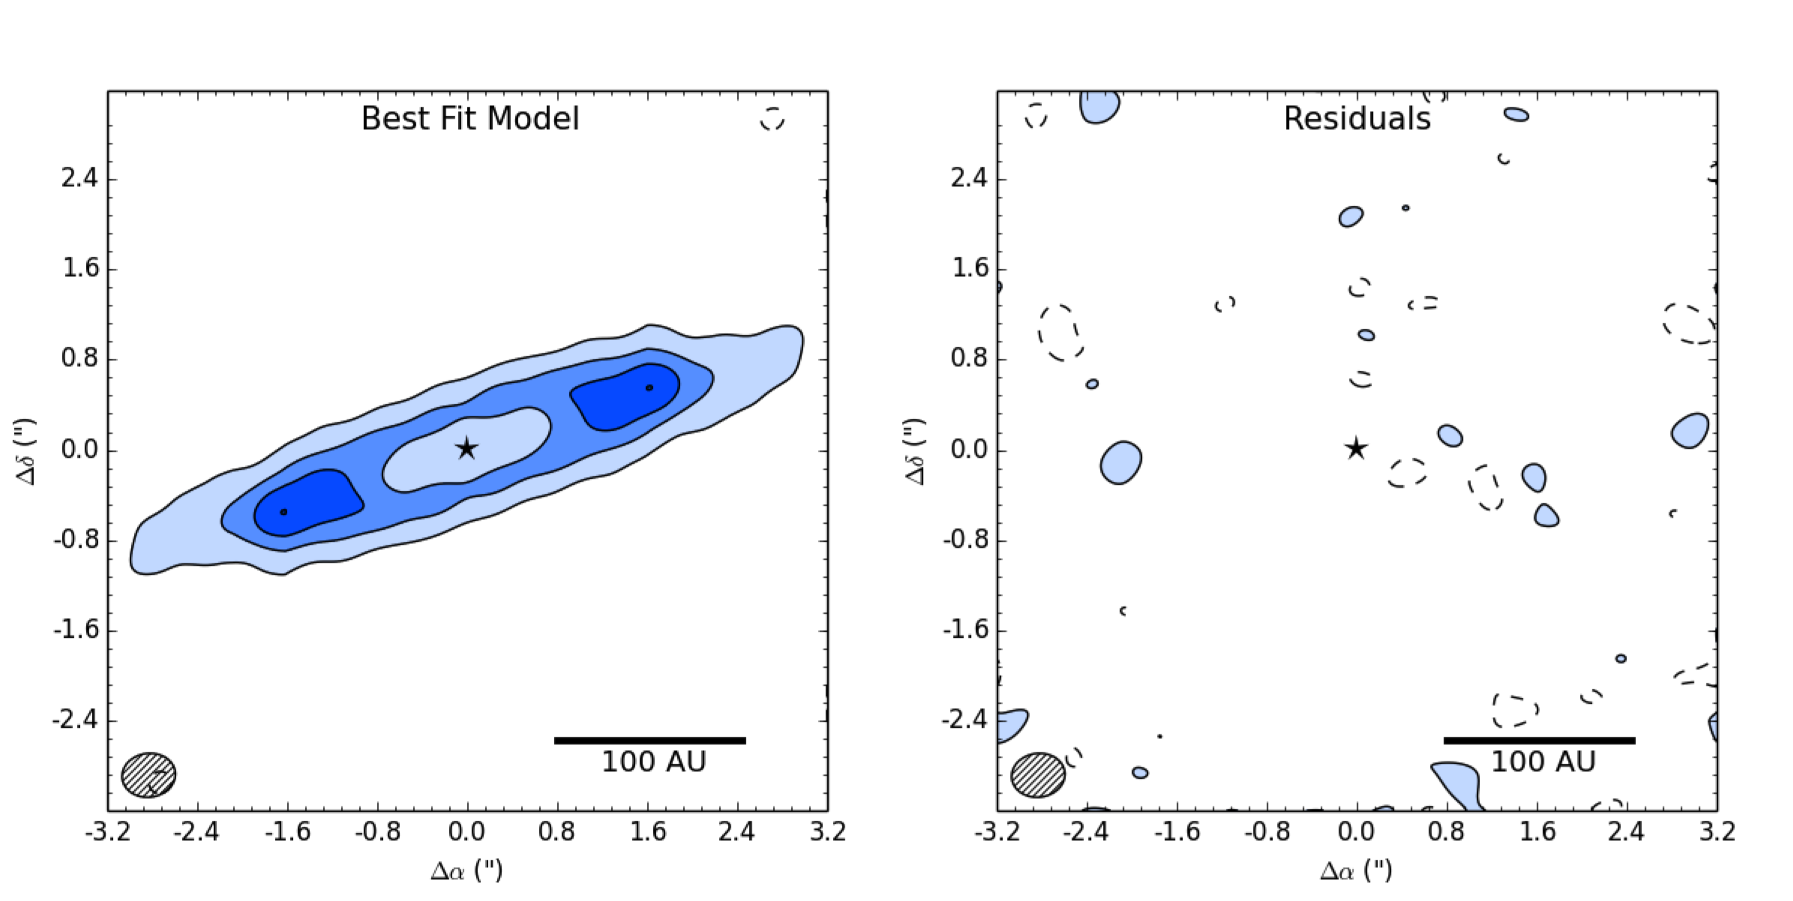
\includegraphics[width = 1\textwidth]{49CET_bBBAG_ModelResidual.png}
\caption{The model image (left) and residuals (right) for the double power law with an an additional inner disk of small grains. Contours are [-2, 2, 4, 6] $\times$ 58$\mu$Jy. The model leaves only a small scatter of 2$\sigma$ residuals. SOMETHING ABOuT NO 2sig in center}
\label{fig:49CET_bBBAG_ModelResidual}
\end{figure}
\end{table}



%%%%

\section{Markov Chain Monte Carlo Simulations}
\label{MCMC}

In order to analyze how successful our models are and explore the uncertainties associated with each parameter, we utilize the affine-invariant Markov chain Monte Carlo (MCMC) fitting technique as described by \cite{Good10} and implemented in Python as \texttt{emcee} by \cite{Fore13}. Using a MCMC method allows us to probabilistically sample the full parameter space described by our models and obtain both a best-fit result and ``most likely" result, and the fact that it is affine-invariant makes it more efficient at sampling degeneracies between parameters. 

This process works by unleashing a series of model ``walkers," with values for parameters in each model sampled as gaussians around a user-stated peak (a best guess, generally) and user-stated width. $\chi^{2}$ values are calculated for each model, and the walkers move around parameter space in search of the best-fit and ``most likely" result for a stated number of steps, with the probability of the move being accepted related to the total $\chi^{2}$ of that model. If the $\chi^{2}$ is lower for the next step, the move is accepted. If the $\chi^{2}$ is higher, the probability of that move being made is $e^{-(\sfrac{\Delta \chi^{2}}{2})}$, with $\Delta \chi^{2}$ = $\chi^{2}_{original}$ - $\chi^{2}_{proposed~model}$. Defined as such, models move toward a best-fit from their original locations in parameter space before filling out a full posterior distribution function for each parameter. The position of each walker in parameter space along with its corresponding $\chi^{2}$ for all steps is called the ``chain," and is saved for further use. 

\begin{figure}
\centering
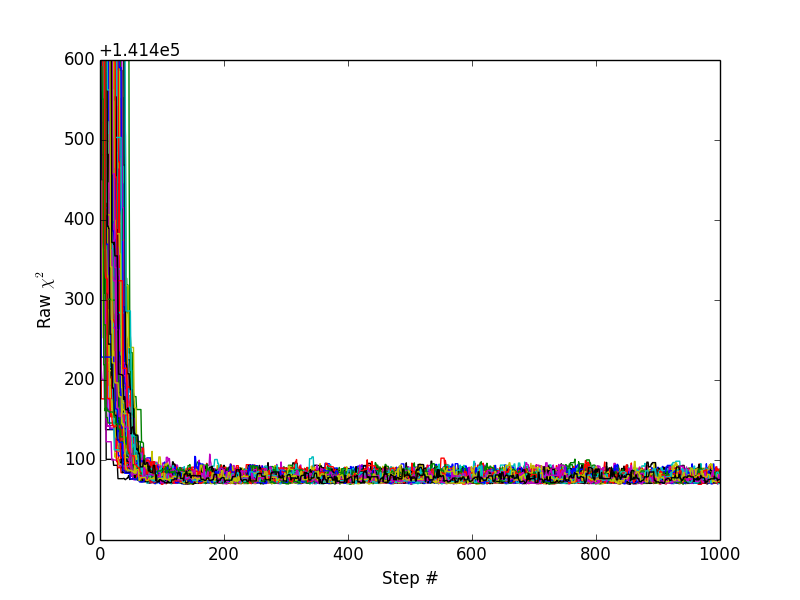
\includegraphics[width = 1\textwidth]{49CET_BurnIn_140x1000_Simplest.png}
\caption{The burn-in and subsequent leveling off of the chi-squared after $\sim$ 100 steps is seen in this plot. Raw $\chi^{2}$ are saved for each step in the chain, and are plotted for each walker (different colors). This burn-in diagram corresponds to the model presented in Section \ref{SinglePowerSED_Model}, which unleashed 140 walkers for 1000 steps.}
\label{fig:49CET_BurnIn}
\end{figure}

\begin{figure}
\centering
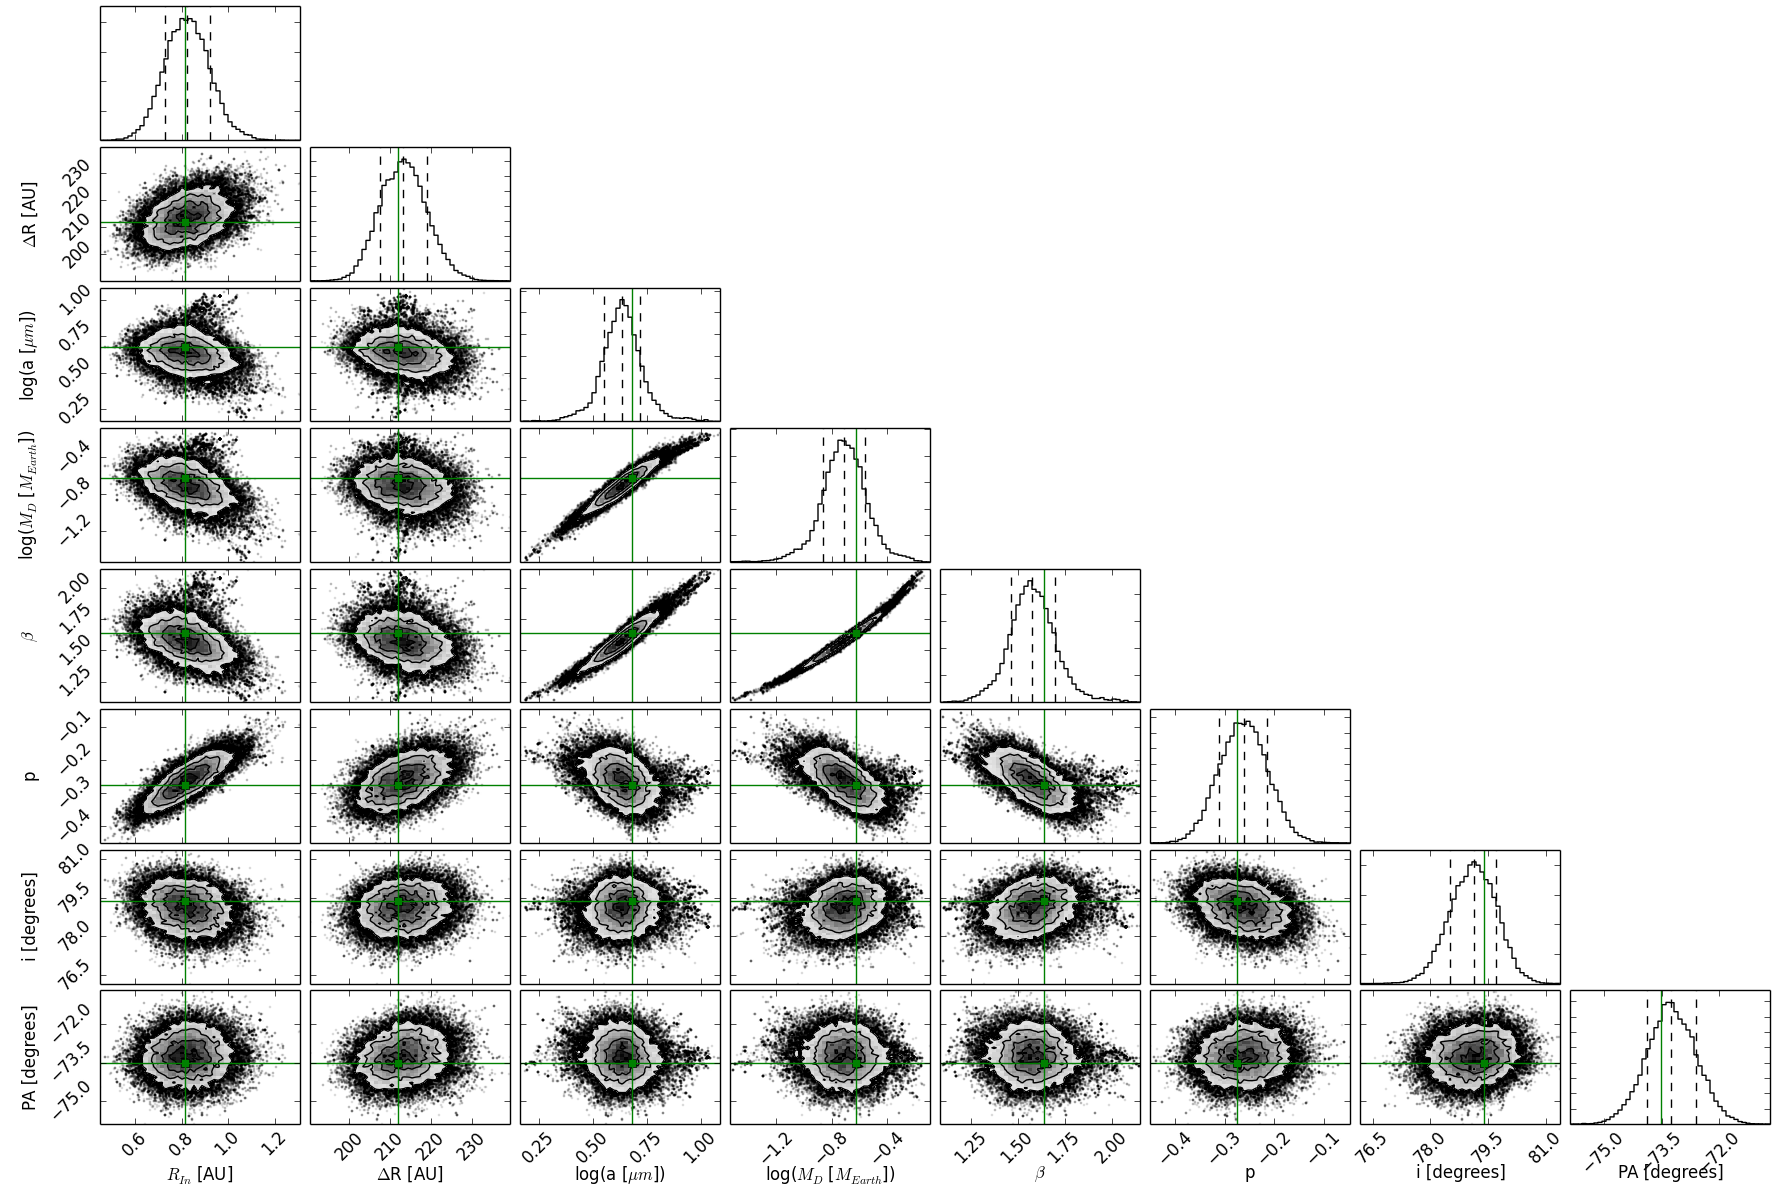
\includegraphics[width = 1\textwidth]{49CET_140x1000_Triangle_150StepBurnIn.png}
\caption{Both one and two dimensional posterior probability distributions for parameters of the single power-law model (Section \ref{SinglePowerSED_Model}) as derived from the MCMC chain. The histograms, along the diagonal, display the marginalized distributions for each parameter independently. The dashed lines in the histogram display -1$\sigma$, the median value, and +1$\sigma$ of the distribution, while the green line displays the value of that parameter associated with the overall minimum $\chi^{2}$. The distributions are mostly symmetric. The median values $\pm1\sigma$ are given in the table in the upper right. The other plots display the two dimensional marginalized distributions for each pair of parameters and demonstrate the covariances between each pair.}
\label{fig:49CET_Triangle}
\end{figure}

The first $\sim$ 100 steps of an MCMC run compromise the ``burn-in" phase, during which the raw $\chi^{2}$ quickly falls as the walkers move toward the best fit (see Fig \ref{fig:49CET_BurnIn}). This phase tends to be longer if the initial value for one or more of the parameters is far from the correct best-fit value. For the first use of a given model, initial MCMC runs were seeded with wide gaussians such that the best-fit is somewhere within and the MCMC process doesn't have a hard time centering in on it. Once a best-fit is known, narrower gaussians are utilized to lessen the burn-in phase. 

The median reported value in each table is the most likely value in the MCMC chain once the burn-in phase has been removed; the best-fit value for each parameter corresponds to the global minimum of the total $\chi^{2}$. As the models trace out posterior distribution functions, values $\pm$ 1$\sigma$ from the median value are also reported. We find that the best-fit values are often within $\pm$ 1$\sigma$ of the median, but this is not always the case. Figure \ref{fig:49CET_Triangle} shows one and two dimensional posterior distributions from the model presented in Section \ref{SinglePowerSED_Model}.

For all models, disk mass parameters ($M_{Disk}$, $M_{Belt}$, etc.) and the grain size $a$ are sampled logarithmically, while the rest of the parameters are sampled in a linear fashion. MCMC runs were computed with $\chi^{2}$ = $\chi^{2}_{Vis}$ + $\chi^{2}_{SED}$ except for the visibility only fits presented in Section \ref{VisOnly}, which had $\chi^{2}$ = $\chi^{2}_{Vis}$. 

\section{Mid-Infrared Properties}
\label{MidIR}

The detail and accuracy of the 360 points that make up the IRS spectrum, presented in Figure \ref{fig:49CET_IRS_Window}, allow us to see characteristic emission features of silicate grains (or the lack thereof). The jump at 14$\mu m$ in the spectrum is not an emission feature, but rather an intrinsic issue due to the fact there are two separate sub-modules being used to take spectra within IRS (one from 5 - 14$\mu m$, the other from 14 - 40$\mu m$). We do not see any emission features at 10$\mu m$, where emission due to silicate grains usually peaks, but this could be due to a variety of possibilities. 
\begin{figure}[t!]
\centering
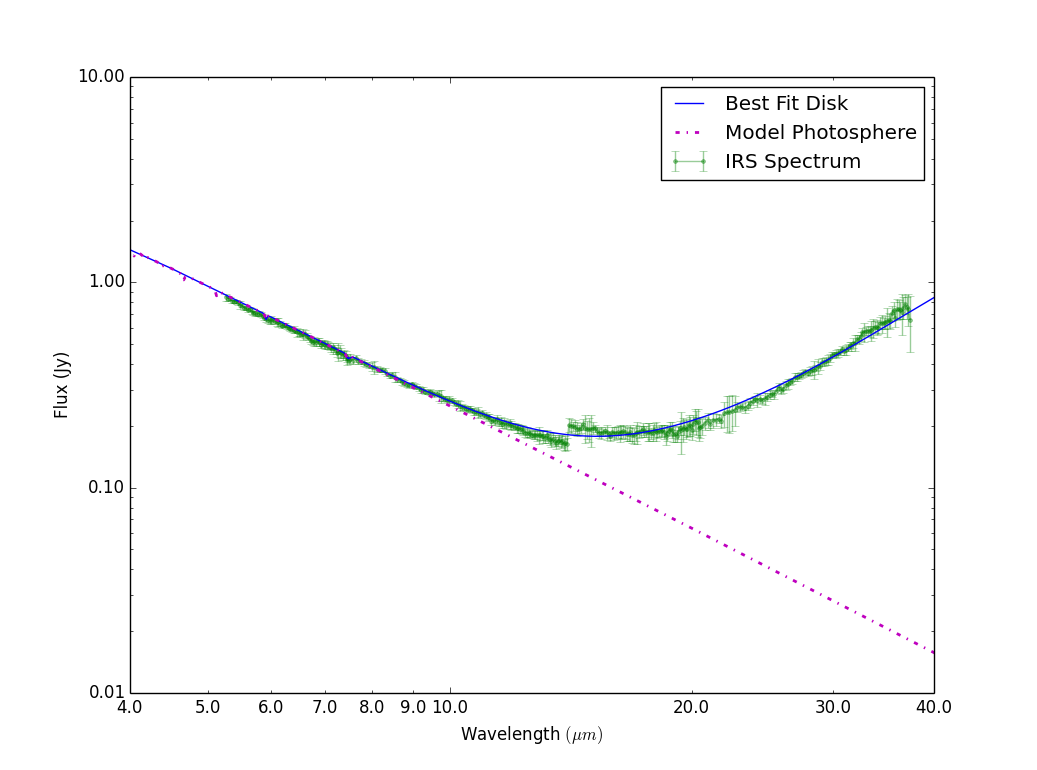
\includegraphics[width = 1\textwidth]{49CET_IRS_Window.png}
\caption{The IRS spectrum of 49 Ceti is plotted in green along with each point's statistical uncertainty. The absolute calibration uncertainty used in fitting the SED, assumed to be 10$\%$ of the flux measurement, is not displayed. A sample best-fit disk and the model photosphere are plotted for reference.}
\label{fig:49CET_IRS_Window}
\end{figure}

Silicate features are most apparent when the emitting grains are smaller than 1$\mu m$ \citep{Papo83}, but can be washed out if they are not the dominant emitters. In addition, even if there are grains of this size, if the crystal lattice structure is uneven, the emission feature will be less pronounced. \cite{Natt07} suggest that the 10$\mu m$ spectral region probes 200-600K grains smaller than a few microns confined to the disk surface within $\sim$ 10AU of the star for protoplanetary disks and within $\sim$ 1AU from the star in the case of T Tauri stars. Our best fit model suggests an inner radius of ?????, which is right on the border of where we expect to find these grains with these characteristics, so it might be that there simply aren't grains with the right properties to display any mid-IR features. 

Finally, it is possible that the percentage of silicate grains is low in 49 Ceti's disk, and that the composition of the grains is dominated by carbonaceous grains. The high albedo of silicate grains is usually responsible for reflecting enough light to be seen in scattered light imaging, but the non-detection of the disk at separations $>$1.6$''$ \cite{Wein99} in scattered light provides evidence that silicates may not dominate the composition. In addition, \cite{Robe14} find an extreme carbon overabundance relative to iron, suggesting that the disk is volatile-rich. However, $\beta$ Pic shows the same overabundance of carbon, but it is easily seen in scattered light with \textit{HST}. 

%Because silicates tend to have much higher albedos than carbon-based grains, the non-detection of any scattered light at separations $>$1.6$''$ \ref{Wein99} suggests that 
%All of these are possibilities for 49 Ceti's disk, but it is unclear what the dominant reason is that we do not observe any silicate features. 


